\chapter{The nucleon-nucleon potential}

Since Chadwick discovered the neutron in 1932, understanding the 
nucleon-nucleon interaction has been a main focus for nuclear physicists.
Yukawa  proposed the first significant theory of the nuclear 
force, see Ref. \cite{yukawa35}, where a meson is exchanged in the 
nucleon-nucleon interaction. This 
meson was later to be identified with the pion. The one pion exchange model
turned out to be very useful in explaining data on nucleon-nucleon scattering
and the properties of the deuteron, see for example Ref. \cite{machleidt2007}. 
Problems arose when multipion exchange were included, and the "pion 
theories" of the 1950's are generally judged to be failures, see for example 
Ref. \cite{machleidt2007}. 
The reasons for the failure of the theories in the 50's is because of the
then unknown pion dynamics understood by QCD and chiral symmetries, which were not to be used by the nuclear physicists until the 80's. 
%The problem of the nuclear force seemed to have been solved by using QCD, however there are still remaining problems such as the nonperturabtive 
%character in the low energy regime.

%The nucleon-nucleon potential is highly repulsive in the short distance as can be seen in Fig(\ref{nucleon_pot}), this repulsive "core" is responsible 
%for why it is prohibitive to do ordinary perturbation theory.
%This problem is circumvented by introducing models containing some of the properties of QCD. All of the realistic models treat the long distance part in 
%a similar manner, by one-pion exchange. They are more varying in the intermediate an short distance part. In this text "$N^3LO$" is the mostly used 
%model. It is derived by chiral perturbation theory, which will be explained below.   
%For a description of various models I refer to Ref. \cite{machleidt-1994-242}.  

\begin{figure}[htp]
\centering
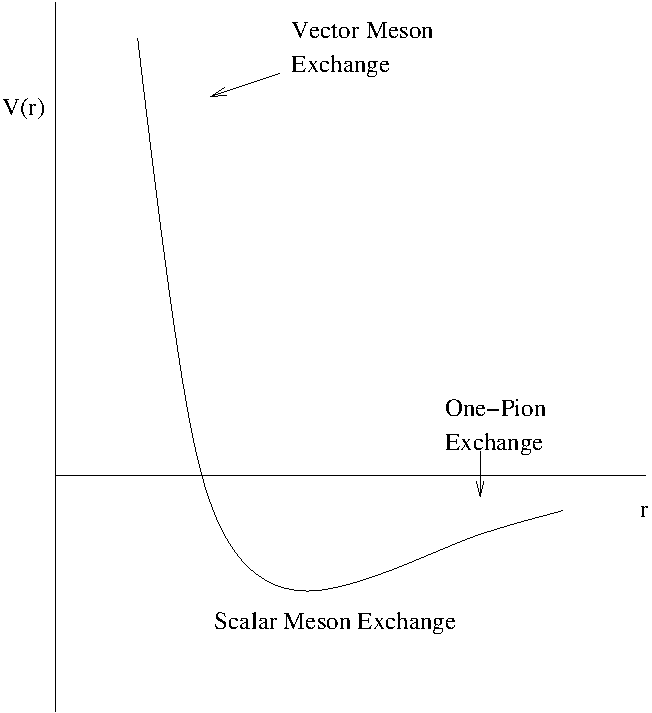
\includegraphics[scale=0.50]{nucleon-nucleon_pot}
\caption{The behavior of the nucleon-nucleon interaction}
\label{nucleon_pot}
\end{figure}

%Fig(\ref{nucleon_pot}) shows the behavior of the nucleon-nucleon interaction, it is repulsive at short distances. 


\section{Chiral Perturbation Theory}

The discovery of QCD and the understanding of effective field theory was a
breakthrough for understanding the nucleon-nucleon potential.\\ QCD is the
theory of the strong interaction, where quarks and gluons are treated as
the degrees of freedom.  The principles behind the theory are really simple and
elegant, the interactions are derived by demanding that the Lagrangian is gauge
invariant under SU(3) group transformations.\\ 
QCD is a non-Abelian field theory as a
consequence of the discovery of the three quantum numbers of color, where the
underlying gauge group is the SU(3) group. QCD is well known for the word "Asymptotic
freedom". With "asymptotic freedom" we say that the 
force governing QCD is weak at short distances but strong, at long distances or
at low energies. The consequences it brings us is that QCD is perturbative at high energies, but non perturbative at low, and that the quarks and gluons 
are confined into "colorless" objects, called hadrons. 
The non-perturbativity of QCD at the low energy regime is 
problematic, the coupling constants are too huge, it becomes meaningless to do a 
perturbative approach since we end up with divergencies at every order of the
expansion parameter. 
As noted earlier, in nuclear physics we operate in this limit, and difficulties arise when treating quarks and gluons
in the nuclear force.  
The solution is to identify the relevant degrees of 
freedom, which in the nuclear case are the nucleons and integrate out the irrelevant ones. 
We treat the nucleons as
"elementary" particles and not as composite of quarks.\\% When identifying the
%nucleons as the degrees of freedom we have to take into consideration the
%properties of the quarks, they will be considered, but hidden in the coupling
%constants.\\
\\
When we do this approximation and construct an effective field theory based on QCD, the symmetries 
of the original Lagrangian must be manifest in the effective Lagrangian. 
In the case of QCD, the Lagrangian is invariant under SU(3) transformations, which also should be a symmetry
of the effective Lagrangian.\\
\\
In the limit where the quark masses are zero, the so-called chiral limit, the 
Lagrangian,
\begin{equation*}
		\mathcal L = \bar q i\gamma^\mu D_\mu q-\frac{1}{4}G^a_{\mu\nu}G^{\mu\nu,a},
\end{equation*}
may be separated into a Lagrangian of left, $q_L,$ and right handed, $q_R$, 
quark fields,
\begin{equation*}
		\bar q_Ri\gamma^\mu D_\mu q_R +\bar q_L i\gamma^\mu D_\mu q_L -\frac{1}{4}G^a_{\mu\nu}G^{\mu\nu,a},
\end{equation*}
where
\begin{equation*}
		q_L=\frac{1}{2}(1-\gamma_5)q=P_Lq~\mbox{and}~ q_R=\frac{1}{2}(1+\gamma_5)q=P_Rq.
\end{equation*}
The chirality matrix $\gamma_5=\gamma^5=i\gamma^0\gamma^1\gamma^2\gamma^3,$ with the properties
\begin{equation*}
		\{\gamma^\mu,\gamma^5\}=0~\mbox{and}~ \gamma_5^2=0,
\end{equation*}
makes the projection operators $P_L$ and $P_R$ satisfy the properties
\begin{equation*}
		P_R^2=P_R,~P_L^2=P_L,
\end{equation*}
and the orthogonality relations
\begin{equation*}
		P_RP_L=P_LP_R=0
\end{equation*}
beside the completeness relation
\begin{equation*}
		P_R+P_L=1.
\end{equation*}
The $\gamma^\mu$ matrices are defined as
\beq
\gamma^0=
\begin{pmatrix}
	I & 0\\
	0&-I
\end{pmatrix}~\mbox{and}~
\gamma^i=\begin{pmatrix}
		0 & \bold \sigma^i\\
		-\bold \sigma^i & 0
		\end{pmatrix},
\eeq
where $I$ is the identity matrix and $\sigma$ the Pauli spin matrices.
The ordinary derivative $\partial_\mu$ is replaced with the covariant derivative
\beq
D_\mu=\partial_\mu-ig\sum_{a=1}^8\frac{\lambda^C_a}{2}\mathcal A_{\mu,a},
\eeq
when we demand invariance under local SU(3) transformations. The SU(3) group transforms by the set eight parameters $\theta$ according to
\begin{equation*}
		q\rightarrow q'=e^{-i\sum_{a=1}^8\Theta_a(x)\frac{\lambda_a^C}{2}}q=U[g(x)]q,
\end{equation*}
where the so-called Gell-Mann matrices $\lambda^a$ are given by
\begin{equation*}
		\lambda^1=
		\begin{pmatrix}
				0&1&0\\
				1&0&0\\
				0&0&0
		\end{pmatrix},~
		\lambda^2=
		\begin{pmatrix}
				0&-i&0\\
				i&0&0\\
				0&0&0
		\end{pmatrix},~
		\lambda^3=
		\begin{pmatrix}
				1&0&0\\
				0&-1&0\\
				0&0&0
		\end{pmatrix},
\end{equation*}
\begin{equation*}
		\lambda^4=
		\begin{pmatrix}
				0&0&1\\
				0&0&0\\
				1&0&0
		\end{pmatrix},~
		\lambda^5=
		\begin{pmatrix}
				0&0&-i\\
				0&0&0\\
				i&0&0
		\end{pmatrix},~
		\lambda^6=
		\begin{pmatrix}
				0&0&0\\
				0&0&1\\
				0&1&0
		\end{pmatrix},
\end{equation*}
\begin{equation*}
		\lambda^7=
		\begin{pmatrix}
				0&0&0\\
				0&0&-i\\
				0&i&0
		\end{pmatrix},~
		\lambda^8=\sqrt{\frac{1}{3}}
		\begin{pmatrix}
				1&0&0\\
				0&1&0\\
				0&0&-2
		\end{pmatrix}.
\end{equation*}
The $G$ denotes the gluon field tensor and $\mathcal A_{\mu,a}$ denotes the 
eight independent gauge potentials.\\
By doing separate left and right handed SU(3) 
transformations
\begin{equation*}
		q_L\rightarrow q'_L=U_Lq_L=e^{-i\sum_{a=1}^8\Theta_a^L\frac{\lambda_a}{2}}q_L,
\end{equation*}
\begin{equation*}
		q_R\rightarrow q'_R=U_Rq_R=e^{-i\sum_{a=1}^8\Theta_a^R\frac{\lambda_a}{2}}q_R,
\end{equation*}
we will see that the Lagrangian remains unchanged and therefore 
is invariant under this transformation,
\begin{equation*}
		\begin{split}
		\mathcal L\rightarrow \mathcal L'=\bar q_RU_R^\dagger U_Ri\gamma^\mu D_\mu q_R +\bar q_LU_L^\dagger U_L i\gamma^\mu D_\mu q_L -\frac{1}{4}G^a_{\mu\nu}G^{\mu\nu,a}=\\
		\bar q_Ri\gamma^\mu D_\mu q_R +\bar q_L i\gamma^\mu D_\mu q_L -\frac{1}{4}G^a_{\mu\nu}G^{\mu\nu,a}=\mathcal L.
\end{split}
\end{equation*}
The quarks have a finite quark mass, but it is not a bad approximation to make them massless
in the nuclear scale since $m_{u,d,s} \ll m_N$, where $u,d,s$ denotes the 
up, down and the strange quark, while $m_N$ stands for the nucleon mass. We will in this chapter only consider the $u$, $d$ and $s$ quarks.\\ 
The remarkable theorem by Emma Noether states that for each symmetry of
the Lagrangian there exists a conserved current.
Let the Lagrangian $\mathcal L(\Phi,\partial_\mu \Phi)$ be invariant under the transformation
\begin{align}
		&    \Phi \rightarrow  \Phi + \alpha\delta  \Phi, \notag
\end{align}
where $\alpha$ is a small parameter.\\
This transformation yields a shift in the Lagrangian,
\begin{align}
		&\alpha\delta \mathcal L=\frac{\partial\mathcal L}{\partial \Phi}\alpha\delta\Phi +\frac{\partial \mathcal L}{\partial(\partial_\mu\Phi)}\alpha\delta(\partial_\mu\Phi)\notag\\
		&= \alpha\Big(\frac{\partial\mathcal L}{\partial \Phi}\delta\Phi-\partial_\mu\frac{\partial \mathcal L}{\partial(\partial_\mu\Phi)}\delta\Phi\Big)+\alpha\partial_\mu\Big(\frac{\partial\mathcal L}{\partial(\partial_\mu\Phi)}\Big)\delta\Phi=\alpha\partial_\mu\big(\frac{\partial\mathcal L}{\partial(\partial_\mu\Phi)}\delta\Phi\big),
		\label{eq:shiftlag}
\end{align}
where we have here made use of the equation of motion 
\begin{align}
	&\Big(\frac{\partial\mathcal L}{\partial \Phi}-\partial_\mu\frac{\partial \mathcal L}{\partial(\partial_\mu\Phi)}\Big)=0.\notag	
\end{align}
When the Lagrangian is invariant under this shift
\begin{align}
	&	\alpha\delta\mathcal L=0=\alpha\partial_\mu\big(\frac{\partial\mathcal L}{\partial(\partial_\mu\Phi)}\delta\Phi\big)=\alpha\partial_\mu J^\mu,
		\label{eq:current}
\end{align}
we have a conserved current $J^\mu$.
In the case of chiral 
invariance the shift in the fields are
\begin{align}
	&	-i\Theta^L_a\frac{\lambda^a}{2}q_L\notag
\end{align}
for the left-handed quark fields and
\begin{align}
	&	-i\Theta^R_a\frac{\lambda^a}{2}q_R\notag
\end{align}
for the right-handed fields. We have neglected terms of order $\Theta_L^2$ and $\Theta_R^2$ and higher.
The eight conserved left-handed currents are 
\beq
L^{\mu,b}=\bar q_L\gamma^\mu\frac{\lambda^b}{2}q_L,  
\eeq
and the eight conserved right-handed currents are
\beq
R^{\mu,b}=\bar q_R\gamma^\mu \frac{\lambda^b}{2}q_R.
\eeq
However these currents can combine to a set of vector currents 
$J^{\mu,b}_V$  and a set of axial currents $J^{\mu , b}_A$, where 
\be
%\begin{split}
 J^{\mu, b}_V=R^{\mu, b} + L^{\mu,b }=\overline q \gamma^\mu \frac{\lambda^b}{2}q 
\ee
and
\be
 J^{\mu,b}_A=R^{\mu, b} - L^{\mu,b }=\overline q \gamma^\mu \gamma_5 \frac{\lambda^b}{2}q.
%\end{split}
\ee
%\begin{equation*}
%		\begin{split}
%				\frac{\lambda^a}{2}=i\frac{\partial}{\partial \theta_a}(0,\cdots,0),\\
%				\lambda^a=\lambda^{\dagger a},\\
%				Tr(\lambda^a\lambda^b)=2\delta_{ab}~\mbox{and}\\
%				Tr(\lambda^a)=0.
%		\end{split}
%\end{equation*}
For each current there is a corresponding conserved charge, Q, which is a generator of $SU(3)_V\times SU(3)_A$.
The conserved charges will in this case be
\beq
%\begin{split}
 Q^b_V=\int d^3xJ^{0,b} \\
\eeq
and
\beq
 Q^b_A=\int d^3xJ^{0,b}_A.
%\end{split}
\eeq
If a mass term, 
\beq
M=
\begin{pmatrix}
		m_u&0&0\\
		0&m_d&0\\
		0&0&m_s
\end{pmatrix},
\eeq
for the quarks is included in the Lagrangian, the symmetry
will break down. Let us look at the QCD Lagrangian with quark masses inserted,
\be
\mathcal L_{QCD}=\overline q(i\gamma^\mu D_\mu - M)q -\frac{1}{4}
G_{\mu \nu}^aG^{\mu \nu,a}.
\ee
The mass term mix the left- and right-handed quark fields
\begin{equation*}
		\bar qMq=\bar q_LMq_R+\bar q_RMq_L.
\end{equation*}
By introducing explicitly the symmetry breaking mass term, the Lagrangian 
nolonger invariant under left- and right-handed SU(3) transformations,
\begin{equation*}
		\bar q_LMq_r+\bar q_RMq_L \rightarrow \bar q_LU_L^\dagger U_RMq_R + 
		\bar q_RU^\dagger_R U_L Mq_L \neq\bar q_LMq_r+\bar q_RMq_L,
\end{equation*}
thus the vector and axial currents are in general not conserved, their divergencies satisfy
\be
\begin{split}
& \partial_\mu J^{\mu,a}_V=i\overline q[M,\frac{\lambda^a}{2}]q\\
& \partial_\mu J^{\mu,a}_A=i\overline q\{\frac{\lambda^a}{2},M\}\gamma_5 q.
\end{split}
\ee
For equal quark masses, the vector currents are conserved since all matrices commute with a multiple of the identity matrix. The axial currents are not
conserved. The symmetry breaks down to $SU(3)_V,$ in the case where the quarks have equal mass.\\
\\
If a symmetry is spontaneously broken, the ground state is no longer
invariant under a certain symmetry, the theory will be enriched by new particles, called
Goldstone bosons. These particles will be massless and have the same quantum numbers as the generators that break the symmetry, see for example Ref.\cite{peskin}.\\
There are reasons to believe that the ground state is not annihilated by the generators of the axial symmetry. If there were an exact axial symmetry we 
would expect the existence of a degenerate hadron multiplet of opposite parity, see for instance Ref.\cite{scherer2005}. For each hadron there should exist a hadron of opposite
parity. These multiplets are not observed, so we assume that the axial symmetry is spontaneously broken and expect eight massless Goldstone bosons. The $SU(3)_V$ is still a valid symmetry when the quarks have equal masses.\\
The involvement of massless Goldstone bosons is problematic, the 
standard model doesn't account for any extra massless particles. This dilemma is
solved by using the fact that the quarks are not massless, this implies that
the Goldstone bosons acquire a small effective mass. The Goldstone bosons are then identified as the pions, kaons and the $\eta$ particles, which have
the same quantum numbers as the broken generators. 
These Goldstone bosons are interpreted as the mediators in the nuclear interactions.

\subsection{The chiral effective Lagrangian}

As mentioned we have to set up an effective Lagrangian containing all the
symmetries of QCD. The chiral effective Lagrangian is given by an infinite
series of terms. The terms contain an increasing number of derivatives. It is
impossible to apply this Lagrangian to nucleon-nucleon scattering, when this
generates an infinite number of Feynman diagrams. Weinberg showed that there is
a systematic expansion of the nuclear amplitude in terms of
\sd(Q/\Lambda_\chi)^\nu\sd, where Q denotes a momentum or pion mass, and
\sd\Lambda\chi\approx 1GeV\sd\, is the chiral symmetry breaking scale. For a
given order \sd\nu\sd\, the number of contributing terms is finite. This scheme
is known as chiral perturbation theory.\\ 	
\\
In order to describe the effective \sd NN\sd\, interaction we write down all terms in the Lagrangian contributing to the given order we want, and consistent with the symmetries. The Feynman diagrams are generated by the terms in the Lagrangian.\\
\\
The effective Lagrangian for \sd NN\sd\, interactions will finally be written as a sum of Lagrangians of pions, nucleons and pion-nucleon interactions
\beq
\mathcal L= \mathcal L_{\pi N}+\mathcal L_{\pi\pi} + \mathcal L_{NN}.
\eeq
These terms are all given by a series of increasing chiral dimension.
\beq
{\cal L}_{\pi N}
=
{\cal L}_{\pi N}^{(1)}
+
{\cal L}_{\pi N}^{(2)}
+
{\cal L}_{\pi N}^{(3)}
+ \ldots ,
\eeq
\beq
{\cal L}_{\pi\pi}
=
{\cal L}_{\pi\pi}^{(2)}
+ \ldots ,
\eeq
\beq
{\cal L}_{NN}
=
{\cal L}_{NN}^{(0)}
+
{\cal L}_{NN}^{(2)}
+
{\cal L}_{NN}^{(4)}
+ \ldots .
\eeq
The superscripts refer to the number of derivatives or pion mass insertions 
\cite{epelbaum2006}.\\
\\
The chiral potential has the form 
\beq
V_{\rm 2N} = V_{\pi} + V_{\rm cont},
\eeq
where $V_{\rm cont}$ denotes the short range term represented by \sd NN\sd\, contact interactions and \sd V_{\rm \pi}\sd\, corresponds to the long range part associated with the pion exchange contribution.
The pion exchange potential may be written as a sum of potentials of different amount of pion exchange
\beq
V_{\pi} = V_{1\pi} + V_{2\pi} + V_{3\pi} + \cdots\,.
\eeq
The two pion exchange potential will not contribute until second leading order 
and the three pion exchange potential will not contribute until fourth order,
\begin{figure}[htb]
%\vspace{-1.0cm}
%\hspace{3.5cm}
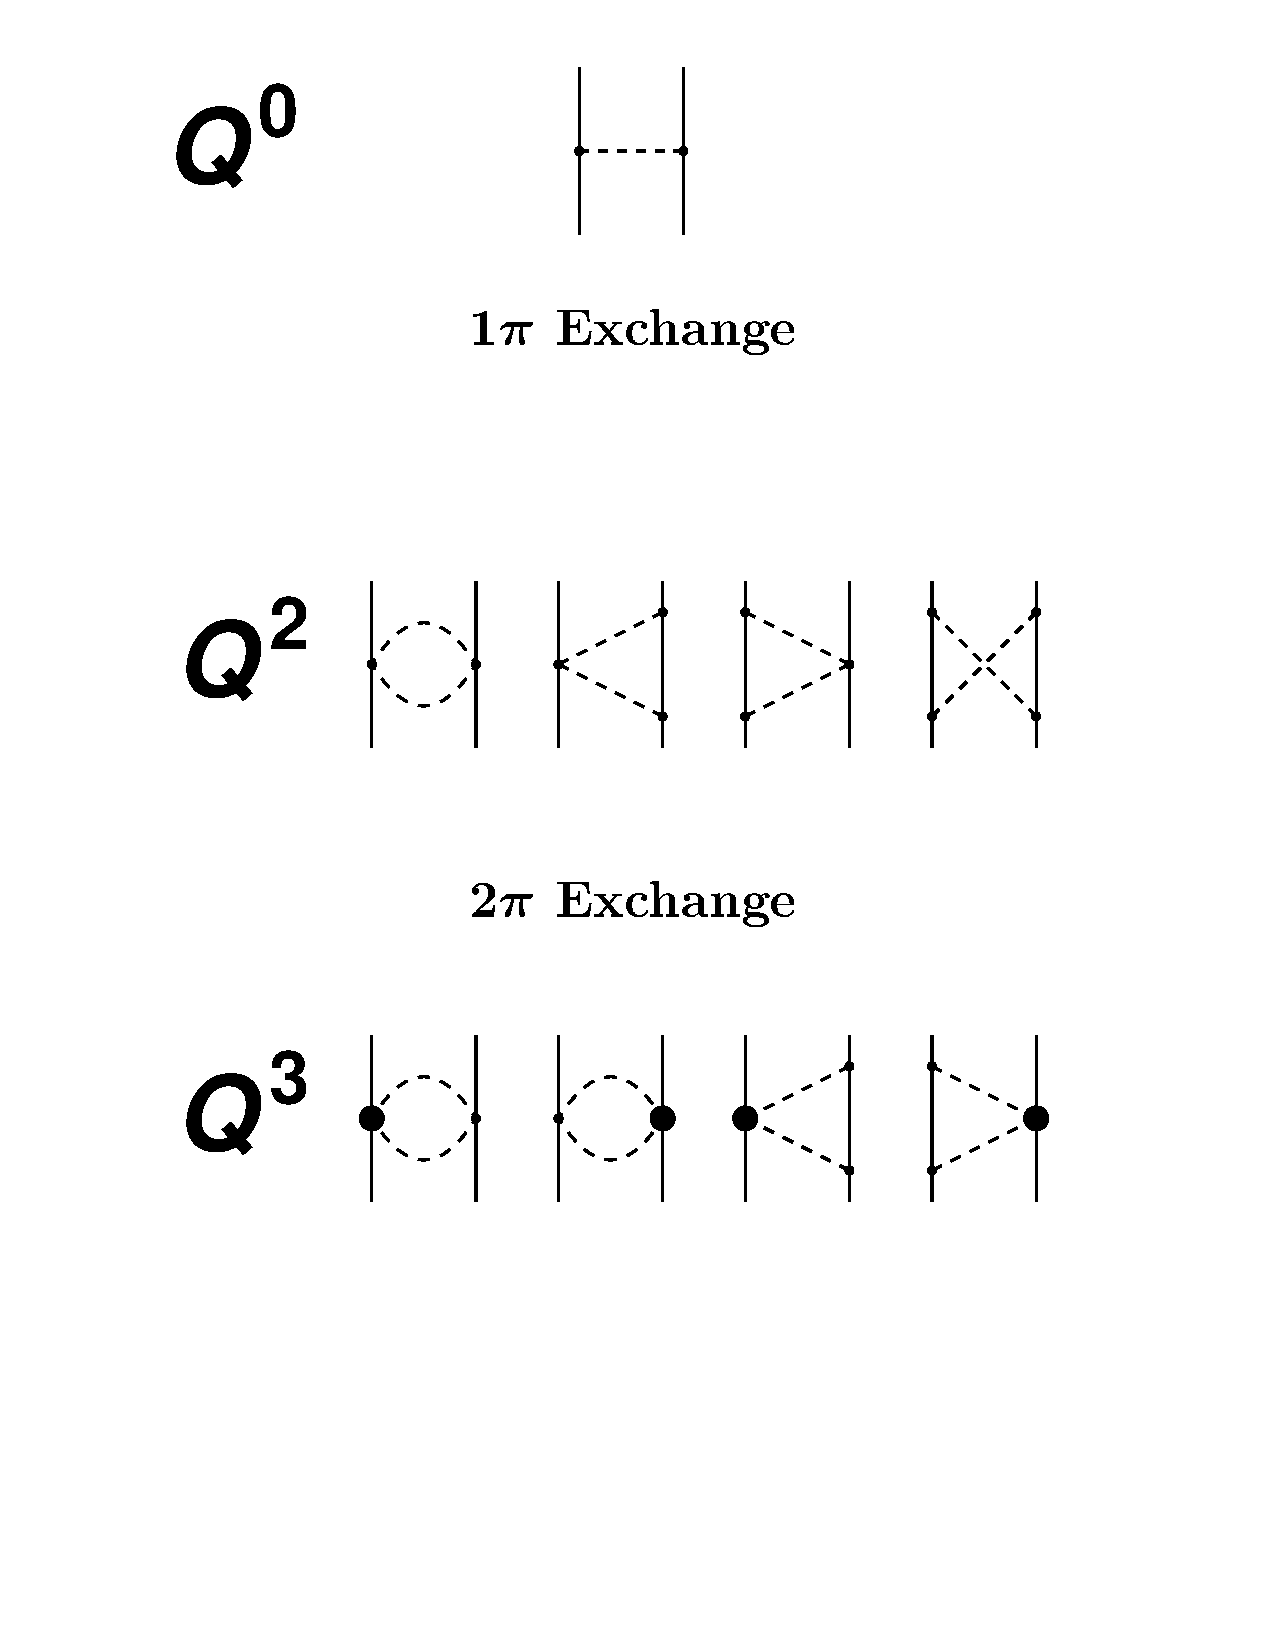
\includegraphics[scale=0.35]{rup1}
%\vspace{-2.5cm}
\caption{The most important irreducible one- and two-pion exchange contributions to the $NN$
interaction up to order $Q^3$. Vertices denoted by small dots are from
$\widehat{\cal L}^{(1)}_{\pi N}$,
while large dots refer to
$\widehat{\cal L}^{(2)}_{\pi N, \, \rm ct}$.}
\end{figure}
\beq
\begin{split}
&V_{1\pi} =   V_{1\pi}^{(0)} +  V_{1\pi}^{(2)} +  V_{1\pi}^{(3)} + V_{1\pi}^{(4
)} + \ldots \,, \\
&V_{2\pi} =   V_{2\pi}^{(2)} +  V_{2\pi}^{(3)} + V_{2\pi}^{(4)} + \ldots \,, \\
&V_{3\pi}  =  V_{3\pi}^{(4)}  + \cdots \,.
\end{split}
\eeq
We notice that $n$--pion  exchange diagrams start to contribute at the order $(Q/\Lambda)^{2n-2}$.\\
\\
The pion exchange potential at N$^3$LO is the sum
\be
V_{1\pi}^{(0)} +  V_{1\pi}^{(2)} +  V_{1\pi}^{(3)} + V_{1\pi}^{(4)}+
+V_{3\pi}^{(4)}.
\ee
  
\section{Derivation of nuclear interactions}

Quantum chromodynamics (QCD)  is the theory which for the moment is believed to
explain the strong interactions among nucleons. The
non-perturbative behavior of QCD in the low energy limit, makes it
difficult to work with. Instead we work with effective field theories. In an
effective field theory, we search for the relevant degrees of freedom, and
integrate out the irrelevant degrees of freedom. In the nuclear limit we use
nucleons and mesons as relevant degrees of freedom, while the quarks and
gluons are frozen out.  In the last section the chiral effective field theory
was briefly explained. And a perturbation series of the nuclear
potential was finally given. How do we derive such potentials? In this section
we will try to derive some meson exchange potentials by using the
phenomenological Lagrangians 
% We need a model to describe the interactions between the nucleons by the
% interchange of mesons. The phenomenological Lagrangians 
\beq
   {\cal L}_{ps} =g^{ps}\overline{\Psi}\gamma^{5}
   \Psi\phi^{(ps)},
   \label{eq:pseudo}
\eeq
\be
   {\cal L}_{s} =g^{s}\overline{\Psi}\Psi\phi^{(s)},
   \label{eq:scalar}
\ee
and
\be
   {\cal L}_{v} =g^{v}\overline{\Psi}\gamma_{\mu}\Psi\phi_{\mu}^{(v)}
   +g^{t}\overline{\Psi}\sigma^{\mu\nu}\Psi\left
   (\partial_{\mu}\phi_{\nu}^{(v)}
   -\partial_{\nu}\phi_{\mu}^{(v)}\right),
   \label{eq:vector}
\ee
for interactions with pseudoscalar mesons, scalar mesons and vector mesons respectively, see Ref. \cite{realeff}.
The coupling constants  $g^{v}$, $g^{t}$, $g^s$ and $g^{ps}$  are purely phenomenological and constrained
from nucleon-nucleon scattering data Ref. \cite{morten:lec1}. 
All the $\phi$'s correspond to the vector, scalar and pseudoscalar mesons, while
$\Psi$ corresponds to the spin 1/2 baryon fields.\\
\\
The baryon fields are the solutions of the Dirac equation
\be
i  \gamma^\mu \partial_\mu \Psi - m  \Psi = 0,
\ee
with the solution 
\be
\Psi (x)={\displaystyle \frac{1}{(2\pi )^{3/2}}
        \sum_{{\bf k}\sigma}u(k\sigma)e^{-ikx}a_{{\bf k}\sigma}},
\ee
where \sd u(k\sigma) \sd are the Dirac spinors
\beq
u(k\sigma)=\sqrt{\frac{E(k)+m}{2m}}
      \left(\begin{array}{c} \chi\\ \\
      \frac{\mbox{\boldmath $\sigma$}{\bf k}}{E(k)+m}\chi
      \end{array}\right), 
\eeq
with $a$ being a fermion annihilation operator and \sd \chi\sd\, the Pauli spinor.
The term $E(k)$ is just the relativistic energy expression.
\beq
E(k) =\sqrt{m^2 +|{\bf k}|^2}
\eeq
With the above Lagrangians and the Feynman diagram rules, see for example 
Refs.\cite{peskin,mandl:qft}, we can derive the two body interaction with interchange of a pion. The vertices are given
by the pseudovector coupling,
\be
V^{pv}=\frac{f_{\pi}^{2}}{m_{\pi}^{2}}\frac{\overline{u}(p_{1}')\gamma_{5}      
\gamma_{\mu}(p_{1}-p_{1}')^{\mu}u(p_{1})\overline{u}(p_{2}')\gamma_{5}
\gamma_{\nu}(p_{2}'-p_{2})^{\nu}u(p_{2})}{(p_{1}-p_{1}')^{2}-m_{\pi}^{2}}.
\ee
The numerator can be further evaluated by using the relationships
\beq
\begin{split}
& \gamma_{\mu}p^{\mu}u(p)=mu(p) \\
& \overline{u}(p)\gamma_{\mu}p^{\mu}=m\overline{u}(p)
\end{split}
\eeq
and  $\{\gamma_{5},\gamma_{\mu}\}=0$, see Refs. \cite{weinberg:qftvol1,Aitchison:gauge}.
Let us calculate the terms involving $p_1$ and $p_1'$ first,
\beq
\begin{split}
&\overline{u}(p_{1}')\gamma_{5}\gamma_{\mu}(p_{1}-p_{1}')^{\mu}u(p_{1})=m\overline{u}(p_{1}')\gamma_{5}u(p_{1})+\overline{u}(p_{1}')\gamma_{\mu}
p_{1}'^{\mu}\gamma_{5}u(p_{1}) \\
&=2m\overline{u}(p_{1}')\gamma_{5}u(p_{1}),
\end{split}
\eeq
The term term involving momenta $p_2$ and $ p_2'$ results in
\beq
\overline{u}(p_{2}')\gamma_{5}\gamma_{\mu}(p_{2}'-p_{2})^{\mu}=
-2m\overline{u}(p_{2}')\gamma_{5}u(p_{1}).
\eeq
We are now able to  write down the coupling in momentum representation as
\be
V^{pv}=-\frac{f_{\pi}^{2}}{m_{\pi}^{2}}4m^{2}\frac{\overline{u}(p_{1}')
\gamma_{5}u(p_{1})\overline{u}(p_{2}')\gamma_{5}u(p_{2})}{(p_{1}-p_{1}')
^{2}-m_{\pi}^{2}}.
\label{eq:vpcouplingmomentum}
\ee
Let us calculate the products $\overline{u}(p')\gamma_{5}u(p)$. By inserting for
the Dirac spinors and the $\gamma_5$ matrix, we see that 
\beq
\begin{split}
&\overline{u}(p_{1}')\gamma_{5}u(p_{1})=\sqrt{\frac{(E_{1}'+m)(E_{1}+m)}
{4m^{2}}}\left(\begin{array}{cc}\chi^{\dagger}-\frac{\sigma_{1}\cdot{
\bf p_{1}}}{E_{1}'
+m}\chi^{\dagger}\end{array}\right)\left(\begin{array}{cc}0&1\\1&0\end{array}
\right)\\
&\times \left(\begin{array}{c}\chi\\ \frac{\sigma_{1}\cdot{\bf p_{1}}}{E_{1}+m}\chi
\end{array}\right)\\
&=\sqrt{\frac{(E_{1}'+m)(E_{1}+m)}{4m^{2}}}\left(\frac{\sigma_{1}\cdot
{\bf p_{1}}}{E_{1}+m}-\frac{\sigma_{1}\cdot{\bf p_{1}'}}{E_{1}'+m}\right). 
\end{split}
\eeq
Similarly, 
\beq
\begin{split}
\overline{u}(p_{2}')\gamma_{5}u(p_{1})=\sqrt{\frac{(E_{2}'+m)(E_{2}+m)}
{4m^{2}}}\left(\frac{\sigma_{2}\cdot {\bf p}_{2}}{E_{2}+m}-
\frac{\sigma_{2}\cdot{\bf p'}_{2}}{E_{2}'+m}\right).
\end{split}
\eeq
It is convenient to operate in the center of mass system, where the total
momentum is zero, \sd p_1=-p_2\sd\, and \sd p_1'=-p_2' \sd\, with \sd
E_1=E_2\sd \, and \sd E_1'=E_2'.\sd\, We can now write down the relativistic contribution, in the
center of mass frame, to the nucleon-nucleon potential, 
\be
\begin{split}
V^{pv}=-\frac{f_{\pi}^{2}}{m_{\pi}^{2}}4m^{2}\frac{1}{(p_{1}-p_{1}')^{2}-
m_{\pi}^{2}}\frac{(E_{1}+m)(E_{1}'+m)}{4m^{2}}\\
\times \left(\frac{\sigma_{1}\cdot{\bf p}_{1}}{E_{1}+m}-\frac{\sigma_{1}
\cdot{\bf p'}_{1}}{E_{1}'+m}\right)\left(\frac{\sigma_{2}\cdot{\bf p}_{1}}
{E_{1}+m}-\frac{\sigma_{2}\cdot{\bf p'}_{1}}{E_{1}'+m}\right).
\end{split}
\label{eq:relativpionpot}
\ee
This work is done in the non relativistic limit, where \sd E=\sqrt{m^2 +p^2}\approx m\sd\, to lowest order.
The energies \sd E_1 \sd\, and \sd E_1'\sd\, are approximately the same. We have
now also an approximation to the non relativistic nucleon-nucleon interaction,
\be
\begin{split}
&V^{pv}=-\frac{f_{\pi}^{2}}{m_{\pi}^{2}}4m^{2}\frac{1}{{\bf k}^{2}+m^{2}}
\frac{2m\cdot 2m}{4m^{2}}\frac{\sigma_{1}}{2m}\cdot({\bf p}_{1}-{\bf p'}_{1})
\frac{\sigma_{2}}{2m}\cdot ({\bf p}_{1}-{\bf p'}_{1})\\
&=-\frac{f_{\pi}^{2}}{m_{\pi}^{2}}
\frac{(\sigma_{1}\cdot{\bf k})(\sigma_{2}\cdot{\bf k})}{{\bf k}^{2}+m_{\pi}^{2}}\tau_1\cdot\tau_2,
\end{split}
\label{eq:nonrelnnint}
\ee
where $\mathbf k$ is the transfered momentum, $(p_{1}-p_{1}')^{2}=-{\bf k}^{2}.$
The $\tau$'s indicate the Pauli isospin matrices.
The exchange terms is omitted.\\
\\
If we want Eq.\eqref{eq:nonrelnnint} expressed in coordinate representation we 
do a Fourier transform of
the equation
\beq
V^{pv}(r)=\int\frac{d^3k}{(2\pi)^3}e^{i{\bf kr}}V^{pv}(k),
\eeq
which results in 
\beq
 V^{pv}(r)=\frac{f_{\pi}^{2}}{m_{\pi}^{2}}\mbox{\boldmath $\tau$}_1\cdot\mbox{\boldmath $\tau$}_2
\sigma_{1}\cdot{\nabla}\sigma_{2}\cdot{\nabla}
\int\frac{d^3k}{(2\pi)^3}e^{i{\bf kr}}\frac{1}{{\bf k}^{2}+m_{\pi}^{2}}.
\eeq
In coordinate representation \sd \bf k \sd\, becomes the differentiation operator \sd \nabla. \sd
The integral over k has to be solved by Cauchy's residue theorem, resulting in
\beq
\begin{split}
&\int\frac{d^3k}{(2\pi)^3}e^{i{\bf kr}}\frac{1}{{k}^{2}+m_{\pi}^{2}}=\int d\Omega \int\frac{dk}{(2\pi)^3}e^{i{kr\cos(\theta)}}k^2\frac{1}{{k}^{2}+m_{\pi}^{2}} \\
&=\int_0 ^\pi d\theta \int\frac{dk}{(2\pi)^2}e^{i{kr\cos(\theta)}}k^2\frac{1}{{k}^{2}+m_{\pi}^{2}}\\ 
&=\int \frac{dk}{ikr(2\pi)^2}(e^{i{kr}}-e^{-ikr})\frac{k^2}{{k}^{2}+m_{\pi}^{2}}=\int \frac{dk}{ir(2\pi)^2}(e^{i{kr}}-e^{-ikr})\frac{k}{({k}+im_{\pi})(k-im_\pi)}\\
&=\frac{e^{-m_{\pi}r}}{2\pi r}.
\end{split}
\eeq
We obtain then
\[
V^{pv}(r)=\frac{f_{\pi}^{2}}{2\pi m_{\pi}^{2}}\mbox{\boldmath $\tau$}_1\cdot\mbox{\boldmath $\tau$}_2
\sigma_{1}\cdot{\nabla}\sigma_{2}\cdot{\nabla}\frac{e^{-m_{\pi}r}}{r}.
\]
Doing the differentiation gives us 
%\beq
%=\frac{f_{\pi}^{2}}{r}e^{-m_\pi r}\mbox{\boldmath $\tau$}_1\cdot\mbox{\boldmath $\tau$}_2{\mbox{\boldmath $\sigma$}_1\cdot\mbox{\boldmath $\sigma$}_2}.
%\eeq
\beq
 \frac{f_{\pi}^{2}}{3\pi }   \left(\sigma_1 \cdot \sigma_2 + \big(1+ \frac{3}{m_\pi r}+ \frac{3}{(m_\pi r )^2}\big)S_{12}\right).
\eeq
Where $S_{12}=(3 \hat r\hat r - \delta_{ij})\sigma_{1}\sigma_{2}$, where $\hat r=\bold r/|r|$.
 To get the full pion exchange nucleon-nucleon potential,
we have to add the exchange term and the isospin dependence.\\
\\
By doing similar derivations for the scalar and vector meson exchange Eqs.
\eqref{eq:scalar} and \eqref{eq:vector},  we get the potential for
exchange of  \sd \omega \sd\, bosons on the form
\be
V^{\omega}= g_{\omega NN}^{2}\frac{1}{{\bf k}^{2}+m_{\omega}^{2}}\left (1-3\frac{{\bf LS}}{2M_N^2}\right).
\ee
For the \sd \rho\sd \, meson the potential becomes 
\be
V^{\rho}= g_{\rho NN}^{2}\frac{{\bf k}^{2}}{{\bf k}^{2}+m_{\rho}^{2}}\left (
-2\sigma_{1}\sigma_{2}+S_{12}(\hat{k})\right)\tau_{1}\tau_{2}.
\ee

\section{$V_{low-k}$}

Since there is a repulsive part in all of the different nucleon-nucleon potentials, even in N$^3$LO, which is derived from the chiral symmetries of QCD, it is necessary to renormalize it. One of the renormalization procedures is called $V_{low-k}$.  This method separates the Hilbert space in a low momentum part and a high momentum part, see Ref. \cite{bogner2003}. This is done by 
introducing a cutoff in momentum space, where all states with momenta higher than the cutoff belong to the high momentum space.\\
\\
As explained above, the nucleon-nucleon interaction
becomes highly repulsive at small interparticle distances. By renormalizing the 
potential the repulsive and the non perturbative part of it "get swept under the
carpet" as Zee in  Ref. \cite{nutshell} says it.
There are many ways to renormalize the potential , or to get "rid off" the high momentum part, all of them must have one thing in common. The renormalized
potential should give an accurate description of the low energy nucleon-nucleon scattering data.\\ %In this case it is $V_{low-k}$ that is used.  
\\
%The nucleon-nucleon interaction has to be treated perturbatively when computing a twobody perturbation diagram. 
The renormalization procedure is based on two steps, see Ref. \cite{gamow} for details. 
The first step is to diagonalize the momentum space for relative momenta. 
We transform $k$ from
$k$~$ \in [0, \infty)$ to $k$~$ \in [0, \lambda ]$,
with a typical value of $\lambda$ approximately $2$ fm$^{-1}$. The renormalized potential, $V_{low-k}$, is dependent on the cutoff.\\
\\
For deriving the effective potential we first have to consider the full 
many-body system described by Schr\" odinger's equation
\be
H\ket{\Psi}=E\ket{\Psi}.
\ee
The Hamiltonian is separated in an unperturbed part and a perturbed part as in chapter \ref{projection}. The separation is written again as
\be
H=H_0+H_I.
\ee
Where $H_I$ denotes the perturbed Hamiltonian and describes the interaction part. 
The first part of constructing an effective Hamiltonian is to use the same projection operators as in chapter \ref{projection}, $P$ and $Q$, that projects onto the low energy state and the high energy state respectively. 
The projection operators still satisfy the properties of Eq.\eqref{projectionopprop}
\beq
\begin{split}
& P^2=P,\\
& Q^2=Q,\\
& P+Q=1,\\
& PQ=QP=0,\\
& [H_0,P]=[H_0,Q]=0\\
\end{split}
\eeq
and
\beq
QH_0P=PH_0Q=0.
\eeq
By using the projection operators the Hamiltonian may be written as 
\be
H=(P+Q)H(P+Q)=PHP+PHQ+QHP+QHQ.
\ee
The Schr\" odinger equation can then be written in  matrix form as
\be
\begin{pmatrix}
PHP & PHQ\\
QHP &QHQ
\end{pmatrix}
\begin{pmatrix}
P\ket{\Psi}\\
Q\ket{\Psi}
\end{pmatrix}
= E
\begin{pmatrix}
P\ket{\Psi}\\
Q\ket{\Psi}
\end{pmatrix}.
\label{effh}
\ee
There exists two main methods for  solving the effective Hamiltonian. The first
is the Bloch-Horowitz \cite{bloch58,blochhoro}, where the effective
Hamiltonian turns out to be dependent on the exact energy eigenvalue one is
solving for. The second method is the so-called Lee-Suzuki method Refs. \cite{suzlee,leesuz}. The
two methods are thoroughly compared in Ref. \cite{jennings-2005-72}.  Both of the
methods result in an effective Hamiltonian on the form 
\be
H_{eff}=PHP
\ee
The solution of the Bloch-Horowitz effective Hamiltonian is
\be
\mathcal H^{BH}_{eff} =P( H +H\frac{1}{E-QHQ}H)P,
\ee
and the corresponding eigenvalue problem 
\be
P( H +H\frac{1}{E-QHQ}H)PP\ket{\Psi}=EP\ket{\Psi}
\ee
has to be solved by a self consistent treatment. \\
\\
The Lee-Suzuki method avoids the difficulties with the energy eigenvalue in the
effective Hamiltonian by doing a similarity transformation of 
the Hamiltonian in Eq. \eqref{effh} to an upper diagonal block matrix as
\be
H^{LS}=
\begin{pmatrix}
P\mathcal H P & P \mathcal H Q\\
0 & Q\mathcal H Q
\end{pmatrix}
=X^{-1}HX
\ee
The condition for $P\mathcal H P$ to be the P space effective Hamiltonian is that
\be
QX^{-1}HXP=0
\label{waveop}
\ee 
The choice of $X$ is crucial, different choices of $X$ lead to different effective
interactions, Lee and Suzuki Ref. \cite{suzlee} made the ansatz of 
\be
\begin{split}
& X=e^\omega\\
& \mathcal H = e^{-\omega}He^\omega,
\end{split}
\label{Eq:omegaeffektiv}
\ee
where $\omega$ is the so-called wave operator. It connects the $P$ and $Q$ 
spaces in the sense that it transform the state
$P\ket{\Psi}$ to the state $Q\ket{\Psi}.$ With the wave operator on the form $\omega=Q\omega P$ the condition \eqref{waveop} is satisfied. This will
also constrain the matrix $X$ by the following properties of the wave operator
\be
\begin{split}
& P\omega P=PQ\omega PP=0, \\
& Q\omega Q=QQ\omega PQ=0,\\
& P \omega Q=PQ \omega QQ=0,\\
\end{split}
\ee
and
\beq
 \omega ^2= Q\omega PQ\omega P=0
\label{waveopconstraint}
\eeq
The expansion of X will then consist of just two terms
\be
X=e^\omega = 1 + \omega=1 + Q \omega P
\ee
The four parts of of the Hamiltonian matrix in \eqref{effh} will then be expressed as 
\be
\begin{split}
& P\mathcal H P=PHP + PH_IQ\omega P,\\
& P\mathcal H Q = PH_IQ,\\
& Q\mathcal H Q= QHQ - \omega PH_IQ,\\
\label{effectivepart}
\end{split}
\ee
and
\beq
 Q\mathcal H P=QH_IP + QHQ\omega - \omega PHP -\omega PH_I Q\omega.
\eeq
With Eq. \eqref{waveopconstraint} and Eq. \eqref{effectivepart} we get an equation for the wave operator such as
\be
QH_IP+QHQ\omega -\omega PHP -\omega PH_IQ\omega = 0.
\label{qhp0}
\ee
If we have a solution for $\omega$, we can insert it in 
Eq.\eqref{Eq:omegaeffektiv} and obtain the effective Hamiltonian 
\be
H_{eff}= PHP + PH_IQ\omega P
\ee
By defining the $P$ space effective interaction operator
\be
V_{eff}=H_{eff}-PH_0P=PH_IP +PH_IQ\omega,
\ee
the $P$ space eigenvalue problem can be written as 
\be
H_{eff}\ket{\psi_\mu}=(PH_0P+V_{eff})\ket{\psi_\mu}=E_\mu \ket{\psi_\mu}.
\ee
The wave operator can be solved in terms of the eigenvalue and eigenstates $E_\mu$ and $\ket{\psi_\mu}$ as
\be
\omega(E_\mu)=\sum_{\mu=1}^d\frac{1}{E_\mu-QHQ}QH_IP\ket{\psi_\mu}\bra{\tilde{\psi}_\mu},
\label{omega}
\ee
where $\bra{\tilde{\psi}_\mu}$ is the bi orthogonal state corresponding to $\ket{\psi_\mu}.$ There are various methods for solving the non-linear equation for the
wave operator. For the two body-problem, we can obtain a desired number of eigenvalues to a given numerical precision. These eigenstates can be used to compute $\omega$.% For more complex systems the equation has to be solved iteratively.  
